\documentclass[11pt,twocolumn,oneside,openany,headings=optiontotoc,11pt,numbers=noenddot]{article}

\usepackage[a4paper]{geometry}
\usepackage[utf8]{inputenc}
\usepackage[T1]{fontenc}
\usepackage{lmodern}
\usepackage[ngerman]{babel}
\usepackage{ngerman}

\usepackage[onehalfspacing]{setspace}

\usepackage{fancyhdr}
\usepackage{fancybox}

\usepackage{rotating}
\usepackage{varwidth}

%Struktogramme
\usepackage[german,curves]{struktex}

\usepackage{pdflscape}
\usepackage{changepage}
\usepackage{graphicx}
\usepackage[bottom]{footmisc}
\usepackage{transparent}
\usepackage{graphbox}
\graphicspath{
	{Pics/PDFs/}
	{Pics/JPGs/}
	{Pics/PNGs/}
}
\usepackage{caption}
\usepackage{wrapfig}
\usepackage{marginnote}
\usepackage{tabularx}
\usepackage{dashrule}
\usepackage{soulutf8}
\usepackage{hhline}
%arydshln suppresses vertical lines in table
%\usepackage{arydshln}
\usepackage{multirow}
\usepackage{enumerate}
\usepackage[hidelinks]{hyperref}
\usepackage{listings}

\usepackage[table]{xcolor}
\usepackage{array}
\usepackage{enumitem,amssymb,amsmath}
\usepackage{interval}
\usepackage{cancel}
\usepackage{stmaryrd}
\usepackage{wasysym}
\usepackage{polynom}
\usepackage{diagbox}
\usepackage{dashrule}
\usepackage{framed}
\usepackage{mdframed}
\usepackage{karnaugh-map}
\usepackage{pdfpages}

\usepackage{blindtext}

\usepackage{eso-pic}

\usepackage{amssymb}
\usepackage{eurosym}

\usepackage[pages=some]{background}
\pagestyle{headings}
\renewcommand{\headrulewidth}{0.2pt}
\renewcommand{\footrulewidth}{0.2pt}
\newcommand*{\underdownarrow}[2]{\ensuremath{\underset{\overset{\Big\downarrow}{#2}}{#1}}}
\setlength{\fboxsep}{5pt}
\newcommand{\explainBelow}[3]{\underbrace{#1}_{\parbox{\widthof{#3}}{\footnotesize\raggedright #2}}}
\newcommand{\explainAbove}[3]{\overbrace{#1}^{\parbox{\widthof{#3}}{\footnotesize\raggedright #2}}}
\newcommand\footnoteref[1]{\protected@xdef\@thefnmark{\ref{#1}}\@footnotemark}


% Codestyle defined
\definecolor{codegreen}{rgb}{0,0.6,0}
\definecolor{codegray}{rgb}{0.5,0.5,0.5}
\definecolor{codepurple}{rgb}{0.58,0,0.82}
\definecolor{backcolour}{rgb}{0.95,0.95,0.92}
\definecolor{deepgreen}{rgb}{0,0.5,0}
\definecolor{darkblue}{rgb}{0,0,0.65}
\definecolor{mauve}{rgb}{0.40, 0.19,0.28}
\colorlet{exceptioncolour}{yellow!50!red}
\colorlet{commandcolour}{blue!60!black}
\colorlet{numpycolour}{blue!60!green}
\colorlet{specmethodcolour}{violet}

%Neue Spaltendefinition
\newcolumntype{L}[1]{>{\raggedright\let\newline\\\arraybackslash\hspace{0pt}}m{#1}}
\newcolumntype{M}{>{\centering\arraybackslash}X}
\newcommand{\cmnt}[1]{\ignorespaces}
%Textausrichtung ändern
\newcommand\tabrotate[1]{\rotatebox{90}{\raggedright#1\hspace{\tabcolsep}}}

%Intervall-Konfig
\intervalconfig {
	soft open fences
}

%Bash
\lstdefinestyle{BashInputStyle}{
	language=bash,
	basicstyle=\small\sffamily,
	backgroundcolor=\color{backcolour},
	columns=fullflexible,
	backgroundcolor=\color{backcolour},
	breaklines=true,
}
%Java
\lstdefinestyle{JavaInputStyle}{
	language=Java,
	backgroundcolor=\color{backcolour},
	aboveskip=1mm,
	belowskip=1mm,
	showstringspaces=false,
	columns=flexible,
	basicstyle={\footnotesize\ttfamily},
	numberstyle={\tiny},
	numbers=none,
	keywordstyle=\color{purple},,
	commentstyle=\color{deepgreen},
	stringstyle=\color{blue},
	emph={out},
	emphstyle=\color{darkblue},
	emph={[2]rand},
	emphstyle=[2]\color{specmethodcolour},
	breaklines=true,
	breakatwhitespace=true,
	tabsize=2,
}
%Python
\lstdefinestyle{PythonInputStyle}{
	language=Python,
	alsoletter={1234567890},
	aboveskip=1ex,
	basicstyle=\footnotesize,
	breaklines=true,
	breakatwhitespace= true,
	backgroundcolor=\color{backcolour},
	commentstyle=\color{red},
	otherkeywords={\ , \}, \{, \&,\|},
	emph={and,break,class,continue,def,yield,del,elif,else,%
		except,exec,finally,for,from,global,if,import,in,%
		lambda,not,or,pass,print,raise,return,try,while,assert},
	emphstyle=\color{exceptioncolour},
	emph={[2]True,False,None,min},
	emphstyle=[2]\color{specmethodcolour},
	emph={[3]object,type,isinstance,copy,deepcopy,zip,enumerate,reversed,list,len,dict,tuple,xrange,append,execfile,real,imag,reduce,str,repr},
	emphstyle=[3]\color{commandcolour},
	emph={[4]ode, fsolve, sqrt, exp, sin, cos, arccos, pi,  array, norm, solve, dot, arange, , isscalar, max, sum, flatten, shape, reshape, find, any, all, abs, plot, linspace, legend, quad, polyval,polyfit, hstack, concatenate,vstack,column_stack,empty,zeros,ones,rand,vander,grid,pcolor,eig,eigs,eigvals,svd,qr,tan,det,logspace,roll,mean,cumsum,cumprod,diff,vectorize,lstsq,cla,eye,xlabel,ylabel,squeeze},
	emphstyle=[4]\color{numpycolour},
	emph={[5]__init__,__add__,__mul__,__div__,__sub__,__call__,__getitem__,__setitem__,__eq__,__ne__,__nonzero__,__rmul__,__radd__,__repr__,__str__,__get__,__truediv__,__pow__,__name__,__future__,__all__},
	emphstyle=[5]\color{specmethodcolour},
	emph={[6]assert,range,yield},
	emphstyle=[6]\color{specmethodcolour}\bfseries,
	emph={[7]Exception,NameError,IndexError,SyntaxError,TypeError,ValueError,OverflowError,ZeroDivisionError,KeyboardInterrupt},
	emphstyle=[7]\color{specmethodcolour}\bfseries,
	emph={[8]taster,send,sendMail,capture,check,noMsg,go,move,switch,humTem,ventilate,buzz},
	emphstyle=[8]\color{blue},
	keywordstyle=\color{blue}\bfseries,
	rulecolor=\color{black!40},
	showstringspaces=false,
	stringstyle=\color{deepgreen}
}

\lstset{literate=%
	{Ö}{{\"O}}1
	{Ä}{{\"A}}1
	{Ü}{{\"U}}1
	{ß}{{\ss}}1
	{ü}{{\"u}}1
	{ä}{{\"a}}1
	{ö}{{\"o}}1
}

% Neue Klassenarbeits-Umgebung
\newenvironment{worksheet}[3]
% Begin-Bereich
{
	\newpage
	\sffamily
	\setcounter{page}{1}
	\ClearShipoutPicture
	\AddToShipoutPicture{
		\put(55,761){{
				\mbox{\parbox{385\unitlength}{\tiny \color{codegray}BBS I Mainz, #1 \newline #2
						\newline #3
					}
				}
			}
		}
		\put(455,761){{
				\mbox{\hspace{0.3cm}
\includegraphics[width=0.2\textwidth]{../../logo.pdf}}
			}
		}
	}
}
% End-Bereich
{
	\clearpage
	\ClearShipoutPicture
}

\setlength{\columnsep}{3em}
\setlength{\columnseprule}{0.5pt}

\geometry{left=1.50cm,right=1.50cm,top=3.00cm,bottom=1.00cm,includeheadfoot}
\pagenumbering{gobble}
\pagestyle{empty}

\begin{document}
	\begin{worksheet}{Mathematik}{Lernabschnitt: Differenzialrechnung}{Extremwertaufgaben}
		\setcounter{section}{7}
		\setcounter{subsection}{5}
		\subsection{Extremwertaufgaben}
		In der realen Welt läuft es bei vielen Problemen technischer, naturwissenschaftlicher, ökonomischer oder mathematischer Art darauf hinaus, dass man eine Fläche, ein Volumen, den Materialverbrauch oder auch die Kosten optimieren möchte.\\
		Hierfür bestimmt man für die entsprechende Funktion einen maximalen oder auch einen minimalen Funktionswert. Diese Berechnung heißt dann \textbf{Extremwertberechnung}.
		\subsubsection{Vorgehensweise}
		Bei der Lösung einer solchen Extremwertberechnung ist es sinnvoll, sich an eine gewisse Vorgehensweise zu halten, damit man keine relevanten Dinge vergisst.
		\subsubsection*{Zeichnen}
		Zunächst verdeutlichen wir uns das Problem, indem wir eine Skizze anfertigen. Diese sollte das gewünschte Ziel ungefähr darstellen.
		\subsubsection*{Hauptbedingung}
		Im nächsten Schritt stellen wir die Anforderung in einer Funktion dar. Diese Funktion entspricht unserer \textbf{Hauptbedingung}. Diese entspricht immer dem Teil, den es gilt zu optimieren (maximieren oder minimieren).
		\subsubsection*{Nebenbedingung(en)}
		Zusätzlich zu der Optimierungsanforderung (Hauptbedingung) liefert die Problemstellung weitere Informationen, welche wir auch in verschiedenen Funktionen darstellen können. Diese Informationen bezeichnen wir als \textbf{Nebenbedingung}. Da das Problem mehrere solcher Informationen aufweisen kann, ist es möglich, dass wir mehrere Nebenbedingungen aufstellen.
		\subsubsection*{Zielfunktion aufstellen}
		Da wir Funktionen mit lediglich einer Variablen lösen können, müssen wir unsere Hauptbedingung mit Hilfe der Nebenbedingungen so umschreiben, dass nur noch \underline{\textbf{eine Variable}} übrig bleibt.\\
		Hierfür stellen wir also unsere Nebenbedingungen nach den korrespondierenden Variablen in der Hauptbedingung um. Anschließend ersetzen wir eben diese Variablen in der Hauptbedingung durch die umgestellten Nebenbedingungen und erhalten damit die gewünschte \textbf{Zielfunktion}.
		\subsubsection*{Definitionsbereich festlegen}
		Um uns die weitere Arbeit zu erleichtern, legen wir als nächstes den Definitionsbereich der Zielfunktion fest. Darunter verstehen wir das Intervall, in dem alle logischen Werte liegen, die die Variable annehmen kann.
		\subsubsection*{Extremwerte berechnen}
		Wir wissen, um das Maximum oder Minimum einer Funktion zu bestimmen, müssen wir die Nullstellen der ersten Ableitung bestimmen.\\
		Das heißt, wir untersuchen die aufgestellte Zielfunktion auf Extremstellen innerhalb des Definitionsbereichs.
		\subsubsection*{Übrige Werte bestimmen}
		Mit Hilfe der errechneten Extremstelle und den zuvor umgestellten Nebenbedingungen können wir nun die weiteren Werte ausrechnen. Hierfür setzen wir die Extremstelle in die Nebenbedingungen ein.
		\subsubsection*{Graphen zeichnen}
		War in der Problemstellung ein Graph mit maximaler oder minimaler Anforderung gefragt, müssen wir diesen zeichnen.
		\subsubsection*{Ergebnis formulieren}
		Abschließend nutzen wir alle berechneten Werte um eine Lösung des Problems zu formulieren.
		\subsubsection*{Beispiel:}
		\begin{framed}
			\noindent
			Mit einem \(20\ cm\) langen Zaun soll für die Meerschweinchen ein größtmögliches rechteckiges Gehege gebaut werden.
		\end{framed}
		\underline{1. Zeichnen}\\
		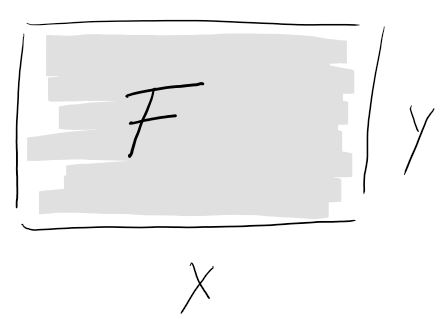
\includegraphics[width=0.35\textwidth]{../99_Bilder/04-6_skizze.jpg}\\
		\underline{2. Hauptbedingung aufstellen}\\
		Wir möchten einen größtmögliches rechteckiges Gehege erhalten.
		\[\mathbf{F = x\cdot{}y}\]
		\underline{3. Nebenbedingung aufstellen}\\
		Im Falle des Drahtes wissen wir, dass dieser nur \(20\ cm\) lang ist. Zudem wissen wir, dass wir eine rechteckige Fläche abstecken müssen. Das bedeutet also
		\[20 = 2\cdot(x+y)\]
		\underline{4. Zielfunktion aufstellen}\\
		Unsere Nebenbedingung lautet \(20 = 2\cdot(x+y)\). Da unsere Hauptbedingung sowohl \(x\) wie auch \(y\) enthält können wir frei entscheiden, nach welcher Variablen wir umstellen.\\
		\begin{tabularx}{0.48\textwidth}{Ml}
			\(20 = 2\cdot(x+y)\) & |\(: 2\)\\
			\(10 = x+y\) & |\(-x\)\\
			\(10 - x = y\)
		\end{tabularx}\\
		\par\noindent
		Diese umgeformte Nebenbedingung setzen wir nun in die Hauptbedingung ein und erhalten \[F = x\cdot(10-x) = \mathbf{-x^2 + 10x}\]
		\underline{5. Definitionsbereich festlegen}\\
		Da wir eine rechteckige Fläche mit den Seitenlängen \(x\) und \(10-x\) erhalten möchten, darf die Variable \(x\) nur Werte im Intervall \[0\ cm \le x \le 10\ cm\] annehmen.\\
		Eine negative Seitenlänge ist nicht möglich und sollte \(x = 0\ cm\) oder \(x = 10\ cm\) betragen, hätten wir kein rechteckiges Gehege.\\
		\underline{6. Extremwerte berechnen}\\
		Für unser Gehege bedeutet das
		\[F' = -2x + 10; E'' = -2\]
		Da die zweite Ableitung negativ ist, können wir direkt Schlussfolgern, dass die berechnete Extremstelle zwangsläufig ein Maximum (Hochpunkt) ist.\\
		\begin{tabularx}{0.48\textwidth}{Xl}
			\(E' = 0\)\\
			\(\Leftrightarrow -2x + 10 = 0\) & |\(+2x\)\\
			\(\Leftrightarrow 10 = 2x\) & |\(:2\)\\
			\(\Leftrightarrow 5 = x\)
		\end{tabularx}\\
		\par\noindent
		Wir wissen nun, dass das Rechteck mit einer Seitenlänge von \(x=5\ cm\) die maximale Fläche hat.\\
		\underline{7. Übrige Werte bestimmen}\\
		Da wir lediglich eine Nebenbedingung haben, müssen wir nur die Breite des Rechtecks berechnen. Für dieses gilt \[y = 10 - \underbrace{5}_{x} = 5\ cm\]
		\underline{8. Lösung formulieren}\\
		Mit einem \(20\ cm\) langen Draht lässt sich eine rechteckiges Gehege mit den Seitenlängen \(x = 5\ cm\) und \(y = 5\ cm\) abstecken.
	\end{worksheet}
\end{document}